% !TEX root = ../0_tcc.tex

\begin{figure}[h]
  \centering
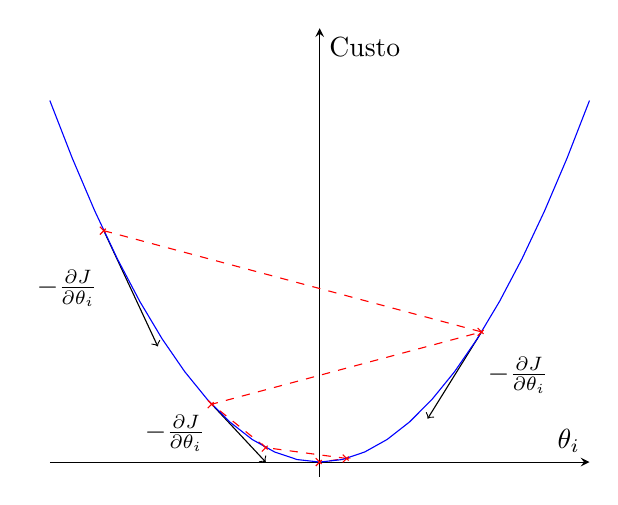
\begin{tikzpicture}
    \begin{axis}[
      clip=false,
      xlabel=$\theta_i$,
      ylabel=Custo,
      xtick={0},
      ytick={0},
      axis y line=center,
      axis x line=middle,
      xmax=5,xmin=-5,
      ymin=-1,ymax=30]

    \addplot[color=red,mark=x,dashed] coordinates {
        (-4,   16)
        (3,     9)
        (-2,    4)
        (-1,    1)
        (0.5,0.25)
        (0,     0)
    };

    \addplot[color=black,->] coordinates {
        (-4,   16)
        (-3,   8)
      } node[pos=0.5, left=0.3cm] {$-\frac{\partial J}{\partial \theta_i}$};

    \addplot[color=black,->] coordinates {
        (3,   9)
        (2,   3)
    }node[pos=0.5, right=0.3cm] {$-\frac{\partial J}{\partial \theta_i}$};

  \addplot[color=black,->] coordinates {
        (-2,   4)
        (-1,   0)
    }node[pos=0.5, left=0.3cm] {$-\frac{\partial J}{\partial \theta_i}$};

    \addplot[blue](x,x*x);

    \end{axis}
\end{tikzpicture}
  \caption{Gradiente descendente em uma função custo quadrática. Fonte: própria.}\label{tikz:gd}
\end{figure}
